\documentclass[a4paper,12pt]{article}
    \usepackage{graphicx}
    \usepackage{indentfirst}
    \title{Combining Fully Convolutional and Recurrent Neural Networks for 3D Biomedical Image Segmentation}
    \author{Jianxu Chen \emph{et al.}}
    \date{2016}

\begin{document}
\maketitle

\section{Contribution}

We propose a new framework combining two DL components: a fully convolutional network (FCN) to extract intra-slice contexts (2D), and a recurrent neural network (RNN) to extract inter-slice contexts (3D).

Comparing to known FCN for 2D biomedical imaging (e.g., U-Net), our new FCN is considerably more effective in dealing with objects of very different scales by simulating human behaviors in perceiving multi-scale information.

Comparing to known RNN models for 3D segmentation, such as Pyramid-LSTM, our RNN model is free of the problematic isotropic convolutions on anisotropic images, and can exploit 3D contexts more efficiently by combining with FCN.

\section{Methodology}

A schematic view of our DL framework is given in Fig. 1. This framework is a combination of two key components: an FCN (called $k$U-Net) and an RNN (called BDC-LSTM).

\begin{figure}[ht]
    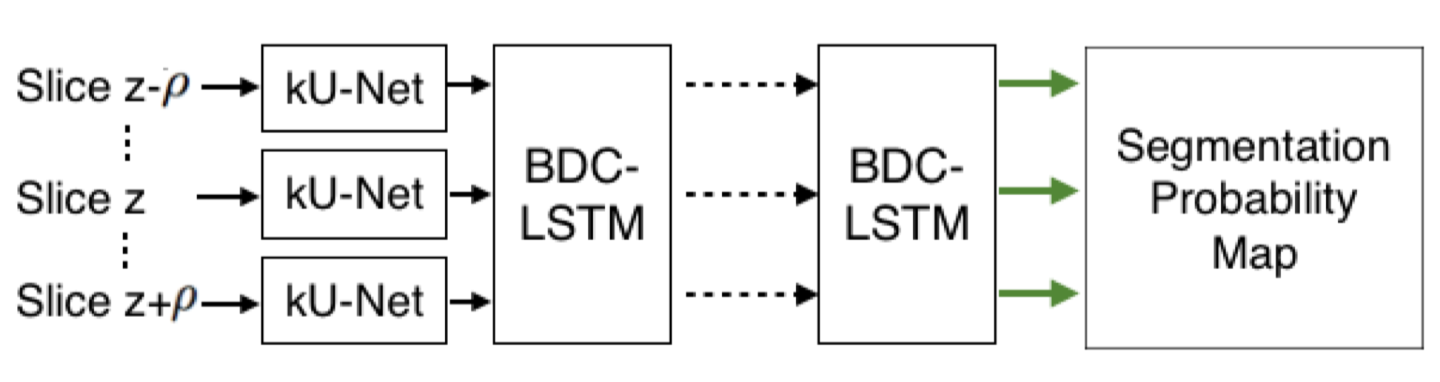
\includegraphics[width=\columnwidth]{img/overview.png}
    \caption{An overview of our DL framework for 3D segmentation. BDC-LSTM, a generalized LSTM network, is applied to a sequence of 2D feature maps, from 2D slice $z - \rho$ to 2D slice $z + \rho$, extracted by $k$U-Nets, to extract hierarchical features from the 3D contexts. Finally, a softmax function (the green arrows) is applied to the result of each slice in order to build the segmentation probability map.}
\end{figure}

\subsection{The FCN Component: $k$U-Net}

We observed that, when human experts label the ground truth, they tend to first zoom out the image to figure out where are the target objects and then zoom in to label the accurate boundaries of those targets.

$k$U-Net employs a sequence of submodule FCNs to extract information at different scales sequentially (from the coarsest scale to the finest scale). The information extracted by the submodule FCN responsible for a coarser scale will be propagated to the subsequent submodule FCN to assist the feature extraction in a finer scale.

\begin{figure}[ht]
    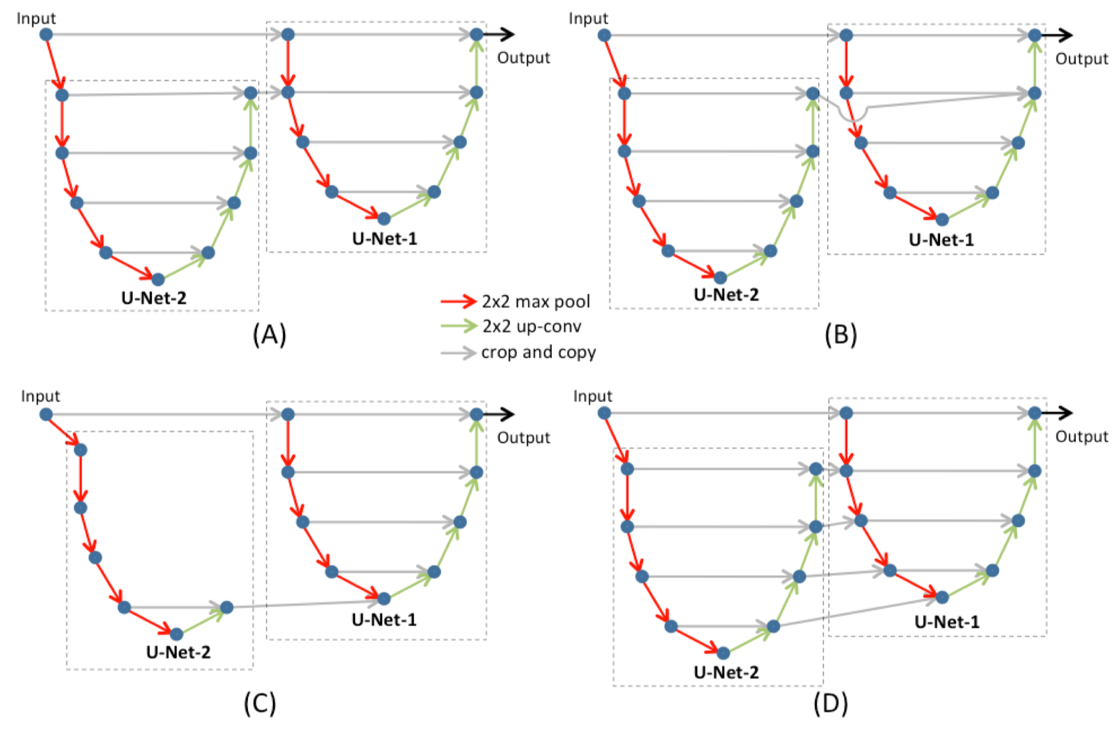
\includegraphics[width=\columnwidth]{img/ku-net.png}
    \caption{Illustrating four different ways to organize $k$ submodule U-Nets in $k$U-Net (here $k = 2$). Architecture (A) is finally adopted for $k$U-Net.}
\end{figure}

Because the parameter $k$ exponentially increases the input window size of the network, a small $k$ is sufficient to handle many biomedical images (we use $k = 2$ in our experiments).

\subsection{The RNN Component: BDC-LSTM}

We extend CLSTM to Bi-Directional Convolutional LSTM (BDC-LSTM). The key extension is to stack two layers of CLSTM, which work in two opposite directions.

To determine the hidden state at a slice $z$, we take the 2D hierarchical features in slice $z$ (i.e., $x_z$ ) and the contextual information from both the $z^{+}$ and $z^{-}$ directions.

Multiple BDC-LSTMs can be stacked into a deep structure by taking the output feature map of one BDC-LSTM as the input to another BDC-LSTM. Besides simply taking one output as another input, we can also insert other operations, like max-pooling or deconvolution, in between BDC-LSTM layers. As a consequence, deep architectures for 2D CNN can be easily migrated or generalized to build deep architectures for BDC-LSTM.

\subsection{Combining $k$U-Net and BDC-LSTM}

Suppose the 3D image consists of $N_z$ 2D slices of size $N_x \times N_y$ each.

\begin{enumerate}
    \item $k$U-Net extracts feature maps of size $64 \times N_x \times N_y$, denoted by $f^z_{2D}$, from each slice $z$. The overlapping-tile strategy (\emph{from U-Net paper}) will be adopted when the 2D images are too big to be processed by $k$U-Net in one shot.
    \item BDC-LSTM works on $f^z_{2D}$ to build the hierarchy of non-linear features from 3D contexts and generate another $64 \times N_x \times N_y$ feature map, denoted by $d^z_{3D}$, $z = 1, \ldots, N_z$. For each slice $z$, $f^h_{2D}$ ($h = z - \rho, \ldots , z, \ldots , z + \rho$) will serve as the context ($\rho = 1$ in our implementation).
    \item A softmax function is applied to $d^z_{3D}$ to generate the 3D segmentation probability map.
\end{enumerate}

\subsection{Training Strategy}

Our whole network, including $k$U-Net and BDC-LSTM, is trained in a decoupled manner. Given the same amount of computing resources (e.g., GPU memory), when allocating all resources to train one component only, both $k$U-Net and BDC-LSTM can take much larger tiles as input.

We use a weighted cross-entropy loss in both the kU-Net and BDC-LSTM training. In biomedical image segmentation, there may often be certain important regions in which errors should be reduced.

\end{document}
